% !TEX root = ../masterthesis.tex
\chapter{Single photon generation using adiabatic rapid passage with frequency-chirped pulses}

\section{Introduction and motivation}

\section{Fundamentals of chirp and adiabatic rapid passage}

A chirped signal is a signal which frequency changes over time.
For example, in a linear-frequency chirp the frequency $f(t)$ would change over time as
\begin{equation}
f(t) = ct+f_0
\end{equation}
where $f_0$ is the starting frequency at $t=0$ and $c$ is the chirpyness. A linear chirped sinusoidal wave is depicted in figure~\ref{fig:chirped-sin}.

\begin{figure}[H]
	\centering
	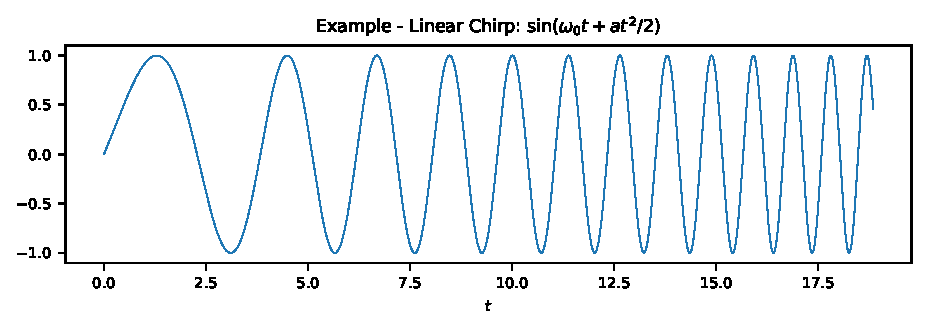
\includegraphics[width=\linewidth]{figures/chirp/chirped-sin}
	\caption{A chirped sinusoidal wave which increases in frequency over time.}
	\label{fig:chirped-sin}
\end{figure}

\todo{Adiabatic rapid passage}
 
\section{Interferometric autocorrelation}

\section{Modified-spectrum autointerferometric correlation}

\section{Adiabatic rapid passage}

\section{Simulation}

\section{Measurements and discussion}